\documentclass[hyperref={bookmarks=false},aspectratio=169]{beamer}
\usepackage[utf8]{inputenc}
\usepackage{standalone}
% ---------------  Define theme and color scheme  -----------------
\usetheme[sidebarleft]{CEIT}  % 3 options: minimal, sidebarleft, sidebarright

%\setbeamertemplate{footline}[frame number]

% ------------  Information on the title page  --------------------
\title[Contents]
{\bfseries{Fundamentals of Computer \& OS Concepts}}

\subtitle{Session 1}

\author[] %\& Managed]
{Josiah Keaton\inst{1} } %\and Managed\inst{2}}

\institute[CEIT]
{
  \inst{1}
  Trainer\\
  Centre of Excellence in IT,PNG
 % \and
 % \inst{2}
 % Trainer\\
 % Centre of Excellence in IT,PNG
}

\date[CEIT, 2014]
{Centre of Excellence in IT, PNG October 2019}
%------------------------------------------------------------

%------------------------------------------------------------
%The next block of commands puts the table of contents at the 
%beginning of each section and highlights the current section:

\AtBeginSection[]
{
  \begin{frame}
    \frametitle{Table of Contents}
    \tableofcontents[currentsection]
  \end{frame}
}

%------------------------------------------------------------


\begin{document}

\frame{\titlepage}  % Creates title page

%---------   table of contents after title page  ------------
\begin{frame}
\frametitle{Table of Contents}
\tableofcontents
\end{frame}
%---------------------------------------------------------


\section{Introduction} 
%---------------------------------------------------------
%Changing visivility of the text
\begin{frame}
\frametitle{Brief Definition and History of Computers}
\begin{exampleblock}{Definition}
	What is a Computer: is programmable electronic device that accepts raw data as input and processes it with a set of instructions (a program) to produce the result as output. It was derived from the Latin word which means, "Compute" - which means to calculate. 
\end{exampleblock}
\begin{large}
	\textbf{History of Computers.}
\end{large}

Generally speaking, computers can be classified into three generations\\
\begin{itemize}
	\item [First generation : 1937 – 1946]
		\begin{itemize}
			\item Developement of the ABC Computer by Developed Dr. John V. Atanasoff and Clifford Berry
			\item 1943 Computer name the Colossus was built for the military
			\item 1946 Electronic Numerical Integrator and Computer (ENIAC) was built
		\end{itemize}
	\item [First generation : ]
\end{itemize}


First generation: 1937 – 1946. Developed Dr. John V. Atanasoff and Clifford Berry and was called called the Atanasoff-Berry Computer (ABC). In 1943 an electronic computer name the Colossus was built for the military. Other developments continued until in 1946 the first general– purpose digital computer, the Electronic Numerical Integrator and Computer (ENIAC) was built.

Second generation: 1947 – 1962 - This generation of computers used transistors instead of vacuum tubes which were more reliable. In 
1951 the first computer for commercial use was introduced to the public; the Universal Automatic Computer (UNIVAC 1). In 1953 the International Business Machine (IBM) 650 and 700 series computers made their mark in the computer world. During this generation of computers over 100 computer programming languages were developed, computers had memory and operating systems. Storage media such as tape and disk were in use also were printers for output.

Third generation: 1963 - present - The invention of integrated circuit brought us the third generation of computers. With this invention computers became smaller, more powerful more reliable and they are able to run many different programs at the same time. In 1980 Microsoft Disk Operating System (MS-Dos) was born and in 1981 IBM introduced the personal computer (PC) for home and office use. Three years later Apple gave us the Macintosh computer with its icon driven interface and the 90s gave us Windows operating system.

As a result of the various improvements to the development of the computer we have seen the computer being used in all areas of life. It is a very useful tool that will continue to experience new development as time passes.
\end{frame}


\begin{frame}
\frametitle{Brief Definition and History of Computers}
\begin{enumerate}
	\setcounter{enumi}{1}
\item Second generation: 1947 – 1962 - This generation of computers used transistors instead of vacuum tubes which were more reliable. In
		\begin{itemize}
			\item 1951 - the first computer for commercial use was introduced to the public Universal Automatic Computer (UNIVAC 1)
			\item 1953 - International Business Machine (IBM) 650 and 700 series. Over 100 computer programming languages were developed, computers had memory and operating systems. Storage media such as tape and disk were in use also were printers for output.
		\end{itemize}
\item Third generation: 1963 - present
		\begin{itemize}
			\item The invention of integrated circuit brought us the third generation of computers. With this invention computers became smaller, more powerful more reliable and they are able to run many different programs at the same time.
			\item 1980 - Microsoft Disk Operating System (MS-Dos) was born and in 1981 IBM introduced the personal computer (PC) for home and office use. Three years later Apple gave us the Macintosh computer with its icon driven interface and the 90s gave us Windows operating system.
		\end{itemize}
\end{enumerate}
\end{frame}

\section{Introduction to Computer Hardare and Softwares} 
%---------------------------------------------------------
%Changing visivility of the text
\begin{frame}

\end{frame}

\section{} 
%---------------------------------------------------------
%Changing visivility of the text
\begin{frame}
\frametitle{Brief History of Computers}
	The computer as we know it today had its beginning with a 19th century English mathematics professor name Charles Babbage.
	He designed the Analytical Engine and it was this design that the basic framework of the computers of today are based on.
	
	Generally speaking, computers can be classified into three generations. Each generation lasted for a certain period of
	time,and each gave us either a new and improved computer or an improvement to the existing computer.
	
	First generation: 1937 – 1946 - In 1937 the first electronic digital computer was built by Dr. John V. Atanasoff and Clifford Berry. It was called the Atanasoff-Berry Computer (ABC). In 1943 an electronic computer name the Colossus was built for the military. Other developments continued until in 1946 the first general– purpose digital computer, the Electronic Numerical Integrator and Computer (ENIAC) was built. It is said that this computer weighed 30 tons, and had 18,000 vacuum tubes which was used for processing. When this computer was turned on for the first time lights dim in sections of Philadelphia. Computers of this generation could only perform single task, and they had no operating system.
	
	Second generation: 1947 – 1962 - This generation of computers used transistors instead of vacuum tubes which were more reliable. In 1951 the first computer for commercial use was introduced to the public; the Universal Automatic Computer (UNIVAC 1). In 1953 the International Business Machine (IBM) 650 and 700 series computers made their mark in the computer world. During this generation of computers over 100 computer programming languages were developed, computers had memory and operating systems. Storage media such as tape and disk were in use also were printers for output.
	
	Third generation: 1963 - present - The invention of integrated circuit brought us the third generation of computers. With this invention computers became smaller, more powerful more reliable and they are able to run many different programs at the same time. In1980 Microsoft Disk Operating System (MS-Dos) was born and in 1981 IBM introduced the personal computer (PC) for home and office use. Three years later Apple gave us the Macintosh computer with its icon driven interface and the 90s gave us Windows operating system.
	
	As a result of the various improvements to the development of the computer we have seen the computer being used in all areas of life. It is a very useful tool that will continue to experience new development as time passes.
\end{frame}



%\begin{frame}
\frametitle{Frame Title 2}
\begin{figure}
    \centering
    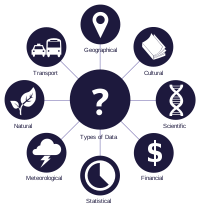
\includegraphics[width=400pt,height=210pt]{figures/fig1.png}
    \caption{``Hollywood is still mad about that, author of \emph{Legends of tech III: Techer In the Dark.}}
    \label{fig:hollywood}
\end{figure}

\end{frame}
%---------------------------------------------------------
%\section{Internet of Things}
\begin{frame}
	\frametitle{Certificate Course in Internet of Things}
	\begin{columns}
		
	\column{0.45\textwidth}
			
		\begin{figure}
			
\includegraphics[width=200pt,height=150pt]{figures/course_iot.jpg}
		\end{figure}
	
	\column{0.55\textwidth}

	\begin{block}{Description}
	
		\begin{enumerate}
			\item Embedded	Linux to develop for IoT. 
			\item Wireless Network \& Communication protocols.
			\item IoT prototyping using NodeJS and Python for development.
			\item Cloud Platforms for IoT.
		\end{enumerate}
	  	  
	\end{block}

	\end{columns}
\end{frame}








%---------------------------------------------------------

%%Two columns
\begin{frame}
\frametitle{Frame Title 4}

\begin{columns}

\column{0.45\textwidth}

\begin{figure}
    \centering
    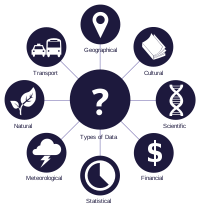
\includegraphics[scale=.4]{figures/fig1.png}
    \caption{``Hollywood is still mad about that, author of \emph{Legends of tech III: Techer In the Dark.}}
    \label{fig:hollywood_prank}
\end{figure}


\column{0.55\textwidth}
In May 1987, undergraduates from Page and Ricketts houses combined forces (and several hundred dollars) to purchase enough black and white plastic, transformed the Hollywood sign to read ``Caltech''.

\small{(Reference: http://www.admissions.caltech.edu/pranks)}

\end{columns}
\end{frame}
%---------------------------------------------------------

%---------------------------------------------------------


\end{document}